\subsection{Separable and inseparable degrees of an extension of finite degree}

Let E be an extension of finite degree of K and \(\Omega\) an algebraic closure of K. Recall (V, p.~31) that by the separable degree of E over K, written \([E:K]_{s}\) , we understand the number of K-homomorphisms of E into \(\Omega\) .

PROPOSITION 15. --- Let \(\mathbf{E}_s\) be the relative separable closure of \(\mathbf{K}\) in \(\mathbf{E}\) ; then \([\mathbf{E}:\mathbf{K}]_s = [\mathbf{E}_s:\mathbf{K}]\) .

The field \(\Omega\) is perfect and \(E\) is \(p\) -radical over \(E_s\) , by \(V\) , p.~44, Prop. 13; therefore Prop. 3 (V, p.~26) shows that every K-homomorphism of \(E_s\) into \(\Omega\) extends in a unique fashion to a K-homomorphism of \(E\) into \(\Omega\) ; we thus have \([E:K]_s = [E_s:K]_s\) . Since \(E_s\) is a separable extension of finite degree of \(K\) , it is an etale algebra over \(K\) ; so we have \([E_s:K]_s = [E_s:K]\) by \(V\) , p.~32, Prop. 4, and the result follows.

With the preceding notation, the degree of E over \(E_{s}\) is called the inseparable degree of E over K and is denoted by \([E:K]_{i}\) . We thus have

\[
[ \mathrm{E}: \mathrm{K} ] = [ \mathrm{E}: \mathrm{K} ] _ {s} \cdot [ \mathrm{E}: \mathrm{K} ] _ {i}\tag{1}
\]

by Prop. 15.

\pandocbounded{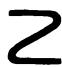
\includegraphics[keepaspectratio]{images/part001_fb7ec604.jpg}}

When K is of characteristic 0, then \(E = E_{s}\) , and so \([E : K]_{s} = [E : K]\) and \([E : K]_{i} = 1\) . If K is of characteristic \(p \neq 0\) , the number \([E : K]_{i}\) is a power of p because E is p-radical over \(E_{s}\) (V, p.~44, Prop. 13 and p.~26, Prop. 4). It should be noted that \([E : K]_{i}\) is not necessarily equal to the highest power of p dividing \([E : K]\) , nor equal to the degree \([E_{r} : K]\) of the relative p-radical closure of E in K (V, p.~152, Ex. 3 and 2).

PROPOSITION 16. --- Let \(\Omega\) be an extension of K and E, F two subextensions of \(\Omega\) , of finite degree over K.

\begin{enumerate}
\def\labelenumi{\alph{enumi})}
\item
  If \(\mathrm{E} \subset \mathrm{F}\) , then \([\mathrm{F}:\mathrm{K}]_s = [\mathrm{F}:\mathrm{E}]_s \cdot [\mathrm{E}:\mathrm{K}]_s\) and \([\mathrm{F}:\mathrm{K}]_i = [\mathrm{F}:\mathrm{E}]_i \cdot [\mathrm{E}:\mathrm{K}]_i\) .
\item
  Let \(\mathbf{K}'\) be a subextension of \(\Omega\) ; then we have
\end{enumerate}

\[
\left[ \mathrm{K} ^ {\prime} (\mathrm{E}): \mathrm{K} ^ {\prime} \right] _ {s} \leqslant \left[ \mathrm{E}: \mathrm{K} \right] _ {s} \quad \text{and} \quad \left[ \mathrm{K} ^ {\prime} (\mathrm{E}): \mathrm{K} ^ {\prime} \right] _ {i} \leqslant \left[ \mathrm{E}: \mathrm{K} \right] _ {i},
\]

and equality holds if \(\mathbf{K}'\) is linearly disjoint from \(\mathbf{E}\) over \(\mathbf{K}\) .

\begin{enumerate}
\def\labelenumi{\alph{enumi})}
\setcounter{enumi}{2}
\tightlist
\item
  We have \([\mathrm{K}(\mathrm{E}\cup \mathrm{F}):\mathrm{K}]_s\leqslant [\mathrm{E}:\mathrm{K}]_s.\) \([\mathrm{F}:\mathrm{K}]_s\) and \([\mathrm{K}(\mathrm{E}\cup \mathrm{F}):\mathrm{K}]_i\leqslant [\mathrm{E}:\mathrm{K}]_i.\) \([\mathrm{F}:\mathrm{K}]_i\) , and equality holds if E and F are linearly disjoint over K.
\end{enumerate}

The assertion about the separable degrees in \(a\) follows from (9) (V, p.~32). Since \([F:K] = [F:E].[E:K]\) , the assertion about the inseparable degrees follows from this and (1).

By Cor. 1 of Prop. 13 (V, p.~44) and Prop. 15, we have

\[
\left[ \mathrm{K} ^ {\prime} (\mathrm{E}): \mathrm{K} ^ {\prime} \right] _ {s} = \left[ \mathrm{K} ^ {\prime} \left(\mathrm{E} _ {s}\right): \mathrm{K} ^ {\prime} \right], \quad \left[ \mathrm{K} ^ {\prime} (\mathrm{E}): \mathrm{K} ^ {\prime} \right] _ {i} = \left[ \mathrm{F} ^ {\prime} (\mathrm{E}): \mathrm{K} ^ {\prime} \left(\mathrm{E} _ {s}\right) \right];\tag{2}
\]

when \(K'\) is linearly disjoint from E over K, then \(E_{s}\) is linearly disjoint from \(K'\) over K and E is linearly disjoint from \(\mathrm{K}'(\mathrm{E}_{s})\) over \(E_{s}\) (V, p.~15, Prop. 8). Assertion b) now follows from Prop. 5 (V, p.~14).

By a) we have \([\mathbf{K}(\mathbf{E}\cup\mathbf{F}):\mathbf{K}]_{s}=[\mathbf{F}(\mathbf{E}):\mathbf{F}]_{s}\cdot[\mathbf{F}:\mathbf{K}]_{s}\) ; by b) we have \([\mathbf{F}(\mathbf{E}):\mathbf{F}]_{s}\leqslant[\mathbf{E}:\mathbf{K}]_{s}\) with equality if E and F are linearly disjoint over K. Hence we obtain the inequality \([\mathbf{K}(\mathbf{E}\cup\mathbf{F}):\mathbf{K}]_{s}\leqslant[\mathbf{E}:\mathbf{K}]_{s}\cdot[\mathbf{F}:\mathbf{K}]_{s}\) with equality if E and F are linearly disjoint over K. The assertion of c) about the inseparable degrees is proved in a similar fashion.

